% ============================================================
\chapter{Introduction aux S\'eries Temporelles}
\label{ch:intro}
% ============================================================

\section{Exemple motivant}
Le cours de cl\^oture journalier de l'indice CAC~40 de 2000 \`a 2024 pr\'esente une tendance, des cycles et une volatilit\'e variable. Contrairement aux donn\'ees iid, chaque observation d\'epend des pr\'ec\'edentes. L'analyse des s\'eries temporelles exploite cette d\'ependance.

\section{D\'efinitions fondamentales}

\begin{definition}[S\'erie temporelle]\index{serie temporelle@s\'erie temporelle}
Une \textbf{s\'erie temporelle} (ou \textbf{processus stochastique \`a temps discret}) est une suite de variables al\'eatoires $(X_t)_{t\in\Z}$ d\'efinies sur un espace de probabilit\'e $(\Omega,\mathcal{F},P)$. Une \textbf{r\'ealisation} (ou trajectoire) est une suite observ\'ee $(x_1,\ldots,x_n)$.
\end{definition}

\begin{definition}[Bruit blanc]\index{bruit blanc}
Un \textbf{bruit blanc} $(\eps_t)$ est une suite de variables al\'eatoires telles que :
\begin{enumerate}
\item $\E[\eps_t]=0$ pour tout $t$,
\item $\Var(\eps_t)=\sigma^2$ pour tout $t$,
\item $\Cov(\eps_t,\eps_s)=0$ pour $t\neq s$.
\end{enumerate}
Notation : $\eps_t\sim\mathrm{BB}(0,\sigma^2)$. Si de plus les $\eps_t$ sont gaussiens, on parle de \textbf{bruit blanc gaussien}.
\end{definition}

\begin{definition}[Bruit blanc fort]\index{bruit blanc!fort}
Un \textbf{bruit blanc fort} est une suite iid de variables al\'eatoires de moyenne nulle et variance finie. Un bruit blanc (faible) n'impose que la d\'ecorr\'elation, pas l'ind\'ependance.
\end{definition}

\section{Composantes d'une s\'erie temporelle}

\begin{definition}[D\'ecomposition classique]\index{decomposition@d\'ecomposition}
On d\'ecompose souvent une s\'erie en :
\[
X_t = T_t + S_t + R_t,
\]
o\`u $T_t$ est la \textbf{tendance} (trend), $S_t$ la \textbf{saisonnalit\'e} (composante p\'eriodique) et $R_t$ le \textbf{r\'esidu} (composante al\'eatoire).

Mod\`ele \textbf{multiplicatif} : $X_t = T_t\cdot S_t\cdot R_t$ (fr\'equent quand l'amplitude saisonni\`ere cro\^it avec le niveau).
\end{definition}

\section{Op\'erateur retard et diff\'erence}

\begin{definition}[Op\'erateur retard]\index{operateur retard@op\'erateur retard}
L'\textbf{op\'erateur retard} $B$ (ou \emph{backshift operator}) est d\'efini par :
\[
BX_t = X_{t-1}, \quad B^k X_t = X_{t-k}.
\]
L'\textbf{op\'erateur diff\'erence} est $\nabla = 1-B$ : $\nabla X_t = X_t - X_{t-1}$.
\end{definition}

\begin{remarque}
On manipule les polyn\^omes en $B$ comme des polyn\^omes ordinaires. Par exemple, $(1-\phi B)X_t = \eps_t$ s'\'ecrit $X_t - \phi X_{t-1} = \eps_t$.
\end{remarque}

\section{Exemples de s\'eries temporelles}

\begin{exemple}[Marche al\'eatoire]\index{marche aleatoire@marche al\'eatoire}
$X_t = X_{t-1} + \eps_t$ avec $\eps_t\sim\mathrm{BB}(0,\sigma^2)$. Alors $X_t = X_0 + \sum_{i=1}^t \eps_i$ et $\Var(X_t) = t\sigma^2 \to \infty$ : la marche al\'eatoire n'est \textbf{pas stationnaire}.
\end{exemple}

\begin{exemple}[Tendance lin\'eaire + bruit]
$X_t = a + bt + \eps_t$. Pas stationnaire (la moyenne $\E[X_t] = a+bt$ d\'epend de $t$).
\end{exemple}

\begin{exemple}[S\'erie saisonni\`ere]
Temp\'eratures mensuelles : p\'eriode $s=12$. On mod\'elise $S_t$ par des fonctions trigonom\'etriques ou des indicatrices mensuelles.
\end{exemple}

\section{Visualisation}

\begin{center}
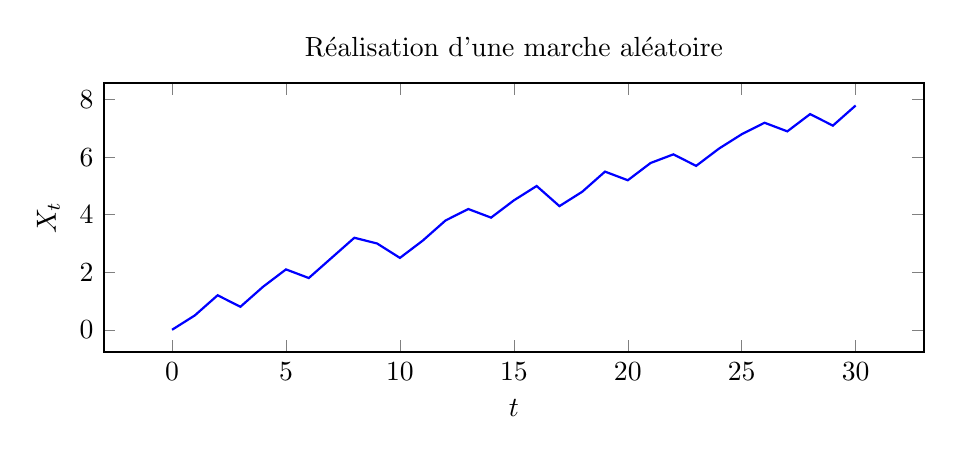
\begin{tikzpicture}
\begin{axis}[
  width=12cm, height=5cm, xlabel={$t$}, ylabel={$X_t$},
  title={R\'ealisation d'une marche al\'eatoire},
  no markers, thick
]
\addplot[blue] coordinates {
(0,0)(1,0.5)(2,1.2)(3,0.8)(4,1.5)(5,2.1)(6,1.8)(7,2.5)(8,3.2)
(9,3.0)(10,2.5)(11,3.1)(12,3.8)(13,4.2)(14,3.9)(15,4.5)(16,5.0)
(17,4.3)(18,4.8)(19,5.5)(20,5.2)(21,5.8)(22,6.1)(23,5.7)(24,6.3)
(25,6.8)(26,7.2)(27,6.9)(28,7.5)(29,7.1)(30,7.8)
};
\end{axis}
\end{tikzpicture}
\end{center}

\begin{center}
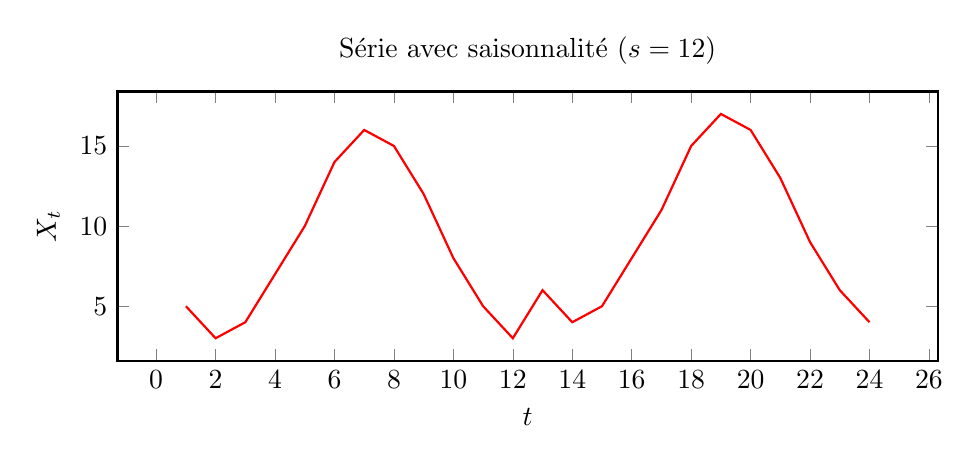
\begin{tikzpicture}
\begin{axis}[
  width=12cm, height=5cm, xlabel={$t$}, ylabel={$X_t$},
  title={S\'erie avec saisonnalit\'e ($s=12$)},
  no markers, thick
]
\addplot[red] coordinates {
(1,5)(2,3)(3,4)(4,7)(5,10)(6,14)(7,16)(8,15)(9,12)(10,8)(11,5)(12,3)
(13,6)(14,4)(15,5)(16,8)(17,11)(18,15)(19,17)(20,16)(21,13)(22,9)(23,6)(24,4)
};
\end{axis}
\end{tikzpicture}
\end{center}

\section{Impl\'ementation}

\begin{codeblock}[title=\textbf{Python}]
\begin{minted}{python}
import numpy as np
import pandas as pd
import matplotlib.pyplot as plt

# Simuler une marche aléatoire
np.random.seed(42)
n = 500
eps = np.random.normal(0, 1, n)
rw = np.cumsum(eps)

# Simuler un AR(1)
phi = 0.8
ar1 = np.zeros(n)
for t in range(1, n):
    ar1[t] = phi * ar1[t-1] + eps[t]

# Charger des données réelles (exemple : AirPassengers)
# url = 'https://raw.githubusercontent.com/jbrownlee/Datasets/master/airline-passengers.csv'
# df = pd.read_csv(url, parse_dates=['Month'], index_col='Month')

fig, axes = plt.subplots(2, 1, figsize=(12, 6))
axes[0].plot(rw, lw=0.8)
axes[0].set_title('Marche aléatoire')
axes[0].set_xlabel('t')

axes[1].plot(ar1, lw=0.8, color='red')
axes[1].set_title('AR(1) avec $\\phi=0.8$')
axes[1].set_xlabel('t')

plt.tight_layout()
plt.savefig('ch01_intro.pdf')
plt.show()
\end{minted}
\end{codeblock}

\section{Exercices}

\begin{exercice}[$\star$]
Simuler 1000 r\'ealisations d'une marche al\'eatoire de longueur $n=200$. Tracer 10 trajectoires sur le m\^eme graphique. Calculer la variance empirique de $X_{200}$.
\end{exercice}

\begin{exercice}[$\star$]
Charger la s\'erie \texttt{AirPassengers}. Identifier visuellement la tendance, la saisonnalit\'e et la volatilit\'e croissante. Proposer un mod\`ele additif ou multiplicatif.
\end{exercice}

\begin{exercice}[$\star\star$]
Montrer que si $X_t = X_{t-1}+\eps_t$ (marche al\'eatoire), alors $\Var(X_t)=t\sigma^2$ et $\Corr(X_t,X_s)=\sqrt{\min(t,s)/\max(t,s)}$ pour $t,s>0$.
\end{exercice}

\begin{exercice}[$\star\star\star$ -- Projet]
T\'el\'echarger les cours journaliers d'une action (ex.\ Apple) sur 5 ans. D\'ecomposer la s\'erie en tendance, saisonnalit\'e et r\'esidu. Calculer les log-rendements $r_t=\ln(P_t/P_{t-1})$ et analyser leurs propri\'et\'es statistiques.
\end{exercice}

\begin{formules}
\begin{align*}
BX_t &= X_{t-1}, \quad \nabla X_t = X_t - X_{t-1} \\
X_t &= T_t + S_t + R_t \quad \text{(d\'ecomposition additive)} \\
\text{Marche al\'eatoire} &: X_t = X_{t-1}+\eps_t, \quad \Var(X_t)=t\sigma^2
\end{align*}
\end{formules}
